%!TEX root = ../thesis.tex
%*******************************************************************************
%*********************************** First Chapter *****************************
%*******************************************************************************

\chapter{Introduction}  \label{c:1} %Title of the First Chapter 

\ifpdf
    \graphicspath{{Chapter1/Figs/Raster/}{Chapter1/Figs/PDF/}{Chapter1/Figs/}}
\else
    \graphicspath{{Chapter1/Figs/Vector/}{Chapter1/Figs/}}
\fi


%********************************** %First Section  **************************************

\epigraph{`[...] there are as many theories of ag[e]ing as there are biogerontologists.'}{L. Hayflick, 2007 \cite{Hayflick2007}}

\section{The biology of ageing} %Section - 1.1 

\subsection{A brief introduction to ageing theory}

The ageing process is one of the most mysterious, complex and fascinating biological problems to be solved in the 21st century. Ageing and immortality have probably fascinated mankind since we have a conception of time and death \cite{Renfrew2016}. 

\bigskip

\textbf{Biological ageing} (\acrshort{a.k.a.} the ageing process) can be broadly defined as the time-dependent functional decline which increases vulnerability to death in most organisms \cite{Lopez-Otin2013}. The revolution taking place in genetics and molecular biology during the 20th century gave rise to more than 300 theories that attempt to explain the mechanisms behind biological ageing \cite{Medvedev1990}. Any valid modern theory of ageing would need to explain at least two things \cite{Medvedev1990}:

\begin{itemize}
	
	\item The molecular basis for the increase in \textbf{mortality rate} (a.k.a. death rate) over time in the population of a given species. Mortality rate can be broadly defined as the number of deaths in a population per unit of time, scaled by the size of the population. More formally, by quantifying the deaths of individuals in a population over time (and assuming that there are no increases in the population number due to reproduction, migration, \acrshort{etc.}), the survival fraction at a given time $t$, $S(t)$, is \cite{Witten1986}:
	
	\begin{align} \label{eq:1.1}
	S(t) = \frac{N(t)}{N_0}
	\end{align}
	
	where $N(t)$ is the number of individuals alive at a given time $t$ and $N_0$ is the initial number of individuals in the population. It can be demonstrated that the mortality rate, $\lambda(t)$, can be expressed as \cite{Witten1986}:
	
	\begin{align} \label{eq:1.2}
	\lambda(t) = - \frac{1}{S(t)} \cdot \frac{dS(t)}{dt}
	\end{align}
	
	\item The \textbf{evolutionary variations in lifespan between different species} \cite{Jones2013}; where lifespan is defined as the time passed between birth and death of an organism. For example, the maximum lifespan in the case of the roundworm (\textit{Caenorhabditis elegans}) is 0.16 years (58.4 days, in captivity); in the case of the fruit fly (\textit{Drosophila melanogaster}) is 0.3 years (109.5 days, in captivity); in the case of the house mouse (\textit{Mus musculus}) is 4 years (in captivity); in the case of humans (\textit{Homo sapiens}) is 122.5 years and in the case of the bowhead whale (\textit{Balaena mysticetus}) is 211 years (in the wild) according to the database AnAge \cite{DEMAGALHAES2009}. Furthermore, some species (such as certain turtles, certain species of rockfish or the bristlecone pine) seem to have negligible senescence \acrshort{i.e.} negligible changes in adult mortality rates over extended periods of time at advanced adult ages \cite{Finch2009}.   
	
\end{itemize}

Nowadays, there are at least \textbf{two main paradigms}, complementary to each other, that try to conceptualise the problem and that are a topic of intense discussion among biogerontologists:

\begin{itemize}
	
	\item Ageing as a consequence of \textit{molecular infidelity}. In this case, stochastic chemical modifications of biomolecules, such as DNA or proteins, exceed the capacity of the repair and turnover systems of the organism and accumulate over time, which increases the entropy of the system. This leads to changes in molecular structure and, finally, changes in function, which increase vulnerability to age-related diseases \cite{Hayflick2007,Hayflick2007a}. From an evolutionary point of view, this fits into the \textit{disposable soma theory}, originally proposed by Thomas Kirkwood in 1977. This theory suggests that organisms have evolved to optimise the amount of energy dedicated to repair errors in somatic cells in order to maximise reproductive success (at the expense of indefinite survival) \cite{Kirkwood1977,Kirkwood1991}. 
	
	\item Ageing as a consequence of \textit{hyperfunction}. In this case, the primary cause of ageing is an excessive activity of certain growth or development-related genes and pathways in later life \cite{Blagosklonny2006,Blagosklonny2010,DeMagalhaes2012,Gems2015}. In other words, ageing originates from developmental programmes that have not been turned off \cite{Blagosklonny2006}. This idea is rooted in the concept of \textit{antagonistic pleiotropy}, an important pillar of the evolutionary theory of ageing originally proposed by George C. Williams in 1957 \cite{Williams1957}. It implies that certain genes have opposite effects on fitness at different ages, which is a consequence of the decrease in selection forces after reproductive age. A strong candidate is the \acrshort{TOR} (target of rapamycin) pathway (see section~\ref{s:1.1.2}), which promotes development in early life but also the advancement of several late-life pathologies \cite{Blagosklonny2010}. 
	
\end{itemize}

It has become clear that no single molecular mechanism will be able to explain ageing across all kingdoms of life. Different species have different life histories that are subjected to evolutionary trade-offs (e.g. regarding reproduction strategies, developmental schedules, etc.) and that can affect the rate of ageing \cite{Jones2013,Ricklefs2010}. Nevertheless, it is possible to integrate all the ideas presented so far into a \textbf{theoretical framework} that can help to unify definitions across studies and set the foundations for mechanistic advancements on the biology of ageing (Fig.~\ref{fig:c1_fig1}, inspired by ideas from \cite{Hayflick2007,Gems2015,Peto1997,Stroustrup2016,Freund2019}). Under this theoretical framework: 

\begin{itemize}
	
	\item The ageing process is composed of different molecular mechanisms (subprocesses) that operate at different stages of life and contribute, in variable proportions, to the appearance of different age-related diseases i.e. the risk of developing an age-related disease is the `integral of its ageing subprocesses operating over time'. Furthermore, the development of different diseases affects the mortality rate and, thus, the probability of dying. The different ageing processes can also be understood as the sources of ageing-associated molecular damage \cite{Lopez-Otin2013}.
	
	\item If the ageing subprocesses can be altered through different genetic, lifestyle or pharmacological interventions, it is possible to reduce the likelihood of several age-related diseases at the same time. This makes ageing research incredibly relevant to the biomedical sciences, since it changes the current paradigm away from developing interventions for a specific already-existing disease towards the prevention of several diseases simultaneously.
	
	\item  Differences in the average lifespan between different species should be explained by different combinations of ageing subprocesses and their rates.
		
\end{itemize}	

\begin{figure}[htbp!] 
	\centering    
	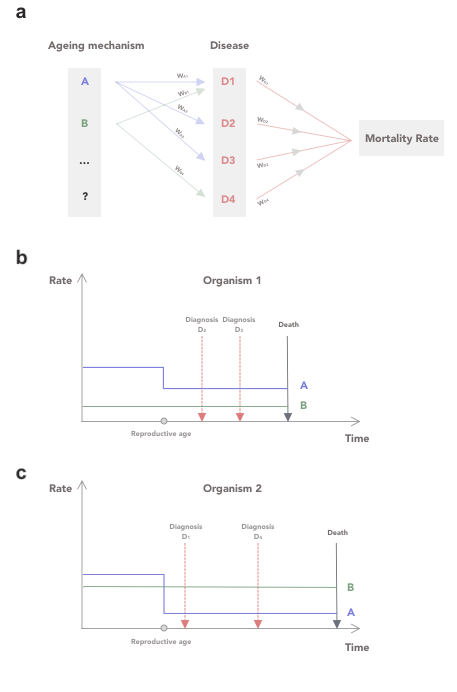
\includegraphics[width=0.8\textwidth]{C1_Fig1}
	\vspace*{1 mm}
	\caption[Theoretical framework to conceptualise the ageing process]{Theoretical framework to conceptualise the ageing process. \textbf{a.} The ageing process is composed of different molecular mechanisms (subprocesses) that operate at different stages of life and contribute, in variable proportions (specified by the weights), to the appearance of different age-related diseases. Furthermore, the development of different diseases affects the mortality rate and, thus, the probability of dying. \textbf{b.} and \textbf{c.} Examples of the life histories of two organisms. In these examples, two ageing mechanisms operate: A (which changes its rate after reproductive age e.g. activated growth-related pathways) and B (with a constant rate over time e.g. some type of (epi)mutational process). Differences in the mechanisms' profiles lead to differences in the age-related diseases that manifest over the lifespan of the organisms, even though the molecular mechanisms are the same. This, affects the mortality rate and, ultimately, the time-to-death. This figure is inspired by ideas from \cite{Hayflick2007,Gems2015,Peto1997,Stroustrup2016,Freund2019}.}
	\label{fig:c1_fig1}
\end{figure}

Consequently, systems biology approaches become fundamental to understand the ageing process \cite{Freund2019}. In the next sections, I will provide an overview of the ageing mechanisms that may operate in different species, with a special focus on mammalian species. 

\smallskip

\subsection{The genetic basis of ageing} \label{s:1.1.2}

\smallskip

Given the large variability in lifespan between species \cite{Jones2013}, it is nowadays clear that the ageing process must have a genetic basis. However, for a long time, the ageing process was thought to be a `haphazard process driven solely by entropy' \cite{Kenyon2005}. Furthermore, in 1935 Clive Maine McCay had shown that caloric restriction (a reduction in calories intake without malnutrition) could extend mean and maximal lifespan in rats \cite{McCay1935,McDonald2010}, which probably shifted the focus towards environmental or external causes as the main driving forces of the ageing process. Since then, dietary restriction (which includes different types of dietary interventions that reduce food intake without malnutrition) has been established as the most successful non-genetic intervention to slow down the ageing process across species \cite{Fontana2015}.

\bigskip

The establishment of the nematode \textit{Caenorhabditis elegans} as a model organism in the 70s triggered its adoption in the ageing field \cite{KLASS1976}, since it allowed well-controlled experiments in a much shorter period of time than rodents \cite{Johnson2013}. This lead to the discovery of the first mutants that dramatically extended lifespan, which mapped to genes in the insulin/IGF-1 signalling pathway \cite{Kenyon1993,Morris1996}. Since then, many genes have been found to significantly affect the lifespan of other model organisms as well, such as in budding yeast (\textit{Saccharomyces cerevisiae}), in fruit flies (\textit{Drosophila melanogaster}) and in mice (\textit{Mus musculus}) \cite{Kenyon2005,Kenyon2010,Singh2019}. 

\bigskip

Interestingly, the effects of many of these genetic mutations and their pathways are shared by distantly-related species. This suggests that at least part of the molecular mechanisms that drive the ageing process could be evolutionarily conserved. Major signalling pathways that have been associated with ageing include the following (Fig.~\ref{fig:c1_fig2}) \cite{Kenyon2005,Kenyon2010,Singh2019,Greer2008}:

\begin{figure}[htbp!] 
	\centering    
	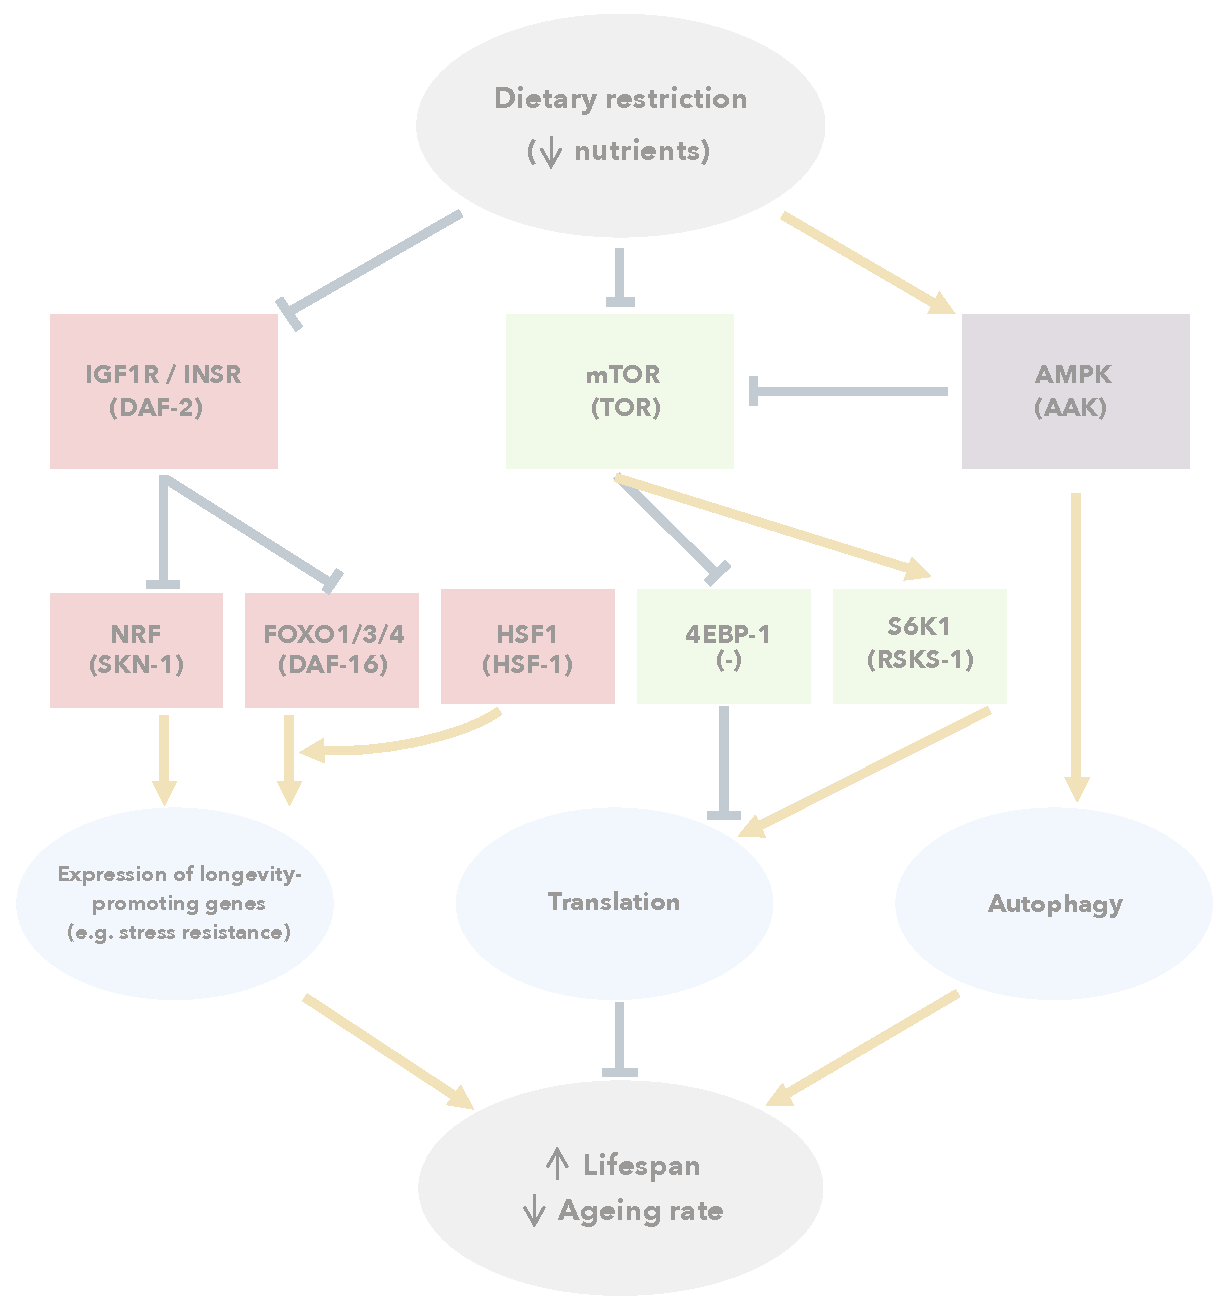
\includegraphics[width=1\textwidth]{C1_Fig2}
	\vspace*{1 mm}
	\caption[Main signalling pathways that affect the ageing process]{Main signalling pathways that affect the ageing process. These pathways sense nutrient and stress inputs (such as a dietary restriction regime) to ultimate impact the rate of ageing. The grey lines represent inhibition (negative regulation) while the yellow arrows represent activation (positive regulation). As such, dietary restriction inhibits the insulin/IGF-1 pathway (in red), inhibits the TOR pathway (in green) and activates AMPK signalling (in purple), ultimately extending lifespan. For simplification, I have only included the main proteins that transduce the signal (e.g. there are more intermediate kinases in the insulin/IGF-1 pathway). Protein names are provided for both the mammalian (top) and the \textit{C. elegans} orthologs if available (bottom, in parenthesis).}
	\label{fig:c1_fig2}
\end{figure}

\begin{itemize} 

	\item \textbf{Insulin/\acrshort{IGF-1} pathway}. This underscores the central role of the endocrine system on the biology of ageing. Mutations that lower the level of \textit{daf-2}, encoding an insulin/IGF-1 receptor, were originally found to double the lifespan of \textit{C. elegans} \cite{Kenyon1993,Guarente2000}. Activation of the insulin/IGF-1 pathway leads to the phosphorylation of a transcription factor of the FOXO family, encoded by \textit{daf-16} in \textit{C. elegans}, which prevents it to reach the nucleus \cite{Lin2001}. FOXO transcription factors, of which there are several members in mammals, activate the expression of longevity-promoting genes involved in processes such as autophagy (which clears protein aggregates and damaged organelles in the cell) \cite{Singh2019}, resistance to oxidative stress or stem cell maintenance \cite{Martins2016}. This partially explains why the inhibition of the insulin/IGF-1 pathway can increase organismal lifespan. However, other downstream targets that regulate gene expression have also been identified, such as \textit{hsf-1} (a transcription factor that regulates heat-shock response) \cite{Hsu2003} or \textit{skn-1} (a transcription factor that coordinates a response to oxidative stress) \cite{Tullet2008} in \textit{C. elegans}.
	
	\item \textbf{\acrshort{TOR} pathway}. \acrshort{TOR} (target of rapamycin) is a kinase that acts as a major amino-acid and nutrient sensor by stimulating growth (including protein translation) and blocking autophagy \cite{Kenyon2010}. The effects of TOR are partly mediated by activating the ribosomal subunit S6 kinase (which promotes protein translation) and by inhibiting 4EBP (a translation inhibitor)  \cite{Kenyon2010,Um2006}. Reductions in TOR activity (via genetic or pharmacological mechanisms) increase lifespan across many species \cite{Kenyon2010}. Importantly, rapamycin, a drug that inhibits TOR, can increase the mean lifespan of mice when fed late in life, which showed for the first time that pharmacological interventions targeting mammalian ageing are possible \cite{Harrison2009}. Interestingly, the increase in lifespan differed in males (9\%) and females (13\%) \cite{Harrison2009}, highlighting the sex-specific effects of some ageing mechanisms. 
	
	\item \textbf{AMPK pathway}. The AMP-activated kinase (\acrshort{AMPK}) controls the balance between catabolic and anabolic processes depending on the cellular levels of \acrshort{AMP}/\acrshort{ATP} (i.e. when ATP levels decrease, AMPK is activated to promote catabolic pathways) \cite{Kenyon2010,Mihaylova2011}. Furthermore, AMPK activation promotes autophagy, partially by inhibiting TOR \cite{Mihaylova2011}. The anti-diabetic drug metformin, which activates AMPK among other targets, has been shown to extend lifespan in mice \cite{Anisimov2008,Martin-Montalvo2013} and has been included as the first drug to target the human ageing process in a clinical trial \cite{Barzilai2016}.
		
	\item \textbf{Sirtuins}. Sirtuins are a family of nicotinamide adenine dinucleotide (\acrshort{NAD$^+$})-dependent deacetylases i.e. they generally catalyse the removal of an acetyl group from lysine residues using \acrshort{NAD$^+$} as a cofactor \cite{Bonkowski2016}. Sirtuins have been shown to play complex roles in the biology of ageing and age-related diseases, in general by cross-talking with other nutrient-sensing pathways and promoting longevity \cite{Kenyon2010,Bonkowski2016}. Several authors have shown that increasing \acrshort{NAD$^+$} levels enhances the activity of sirtuins, which could constitute an additional anti-ageing pharmacological avenue in mammals. Additionally, intensive research is being carried out to identify other molecules that activate sirtuins \cite{Bonkowski2016}.
	
	\item \textbf{Other pathways}. Mitochondrial respiration (and its production of reactive oxygen species or \acrshort{ROS}), genome surveillance pathways (such as those involved in DNA repair or telomere maintenance), signals from the reproductive system or Wnt signalling have also been implicated in different ways in the ageing process \cite{Kenyon2010,Greer2008, Lezzerini2014}.
	
\end{itemize}


These pathways seem to have a dual role depending on the environmental context that the organism is facing, behaving as \textbf{nutrient and stress sensors}. Under abundant nutrient availability and low stress (oxidative, temperature), they tend to promote growth and reproduction. While in contrast, under harsh conditions (such as those posed by dietary restriction), they favour cell protection and maintenance \cite{Kenyon2005,Kenyon2010}. It is worth mentioning that the responses of the different pathways to dietary restriction deeply depend on the characteristics of the diet and its timing \cite{Kenyon2010}. This model also relates to the disposable soma theory, where more resources are allocated either to reproduction or somatic maintenance depending on the context \cite{Kirkwood1977,Kirkwood1991}. This is further mechanistically supported by experiments showing that decreased insulin/IGF-1 signalling (e.g. via \textit{daf-2} mutation) produces the acquisition of germline characteristics (e.g. higher genomic stability) in \textit{C. elegans} somatic cells \cite{Curran2009}. Even though this model is a clear oversimplification, it becomes useful when thinking about the way in which the ageing process might have evolved and how the same biological pathways can be repurposed to activate genetic programs with completely different goals.

\bigskip

There are many more \textbf{complexities associated with these pathways} that would require an entire thesis on its own. For example, the insulin/IGF-1 signalling pathway can work in a cell non-autonomous manner (i.e. the activity of the pathway in one tissue can affect lifespan by influencing cells in a different tissue), which could help to coordinate ageing rates in the organism, and the effects are many times tissue-specific \cite{Kenyon2005,Kenyon2010}. Additionally, the pathways can have different effects depending on the life stage of the animal (e.g. development, adulthood, etc.) \cite{Dillin2002}. Furthermore, cross-talk between the pathways has previously been reported \cite{Bonkowski2016, Greer2007}. Therefore, the inner workings of these signalling pathways is still an area of intense research.

\bigskip

The discovery of signalling pathways that can dramatically extend the lifespan of model organisms has demonstrated that \textbf{the ageing process has a genetic basis and it is possible to alter its rate}. More importantly, the appearance of age-related disease seems to be delayed in many of these long-lived organisms \cite{Kenyon2010,Arantes-Oliveira2003}, suggesting that these interventions indeed reduce the rate of some the operating ageing mechanisms (Fig.~\ref{fig:c1_fig1}). 

\smallskip

\subsection{Hallmarks of mammalian ageing} \label{s:1.1.3}

\smallskip

Most studies on the biology of mammalian ageing have been conducted in mice. Many genetic mutations in conserved pathways (mainly nutrient-sensing pathways) have been shown to significantly extend the lifespan of mice. Among them, those that affect growth hormone signalling (which in mammals in turn controls the secretion of IGF-1 by the liver and therefore the insulin/IGF-1 signalling pathway) produce the longest lifespan improvements (in the order of 40-60\%) \cite{Singh2019}. Even though this is a remarkable result, it is far off the lifespan extensions achieved with `simpler' model organisms such as \textit{C. elegans} (where extensions of almost 1000\% have been achieved with a mutation in a single gene of the insulin/IGF-1 pathway; the equivalent of a human living up to $\approx 1200$ years!) \cite{Ayyadevara2008}. This highlights a trend where translating lifespan interventions discovered in worms and flies yields generally less spectacular results in mice and potentially in humans.

\bigskip

Evolution has been experimenting with lifespan extension for a long time. Consequently, some species of mammals, such as the naked mole rat (\textit{Heterocephalus glaber}) or some species of bats (Chiroptera), are exceptionally long-lived for their body size. Recent reports point towards the possibility that these species do not increase their mortality rate with age (i.e. they may have negligible senescence) \cite{Ruby2018,Fleischer2017}, which makes them incredibly interesting systems to study the biology of ageing in mammals. 

\bigskip

In 2013, L\'opez-Ot\'in \textit{et al.} reviewed the main common denominators of the ageing process across organisms \cite{Lopez-Otin2013}. They defined several \textbf{hallmarks of ageing}, which can be understood as the measurable consequences of the ageing mechanisms that I proposed in Fig~\ref{fig:c1_fig1}. I will briefly discuss some of them, with a special focus on those that directly affect the genome during mammalian ageing  \cite{Lopez-Otin2013,Singh2019}:

\begin{itemize}
	
	\item \textbf{Genomic instability}. Somatic DNA mutations (single nucleotide variants, copy number changes, structural rearrangements, etc.) accumulate over time in mammalian cells (both in the nuclear genome and the mitochondrial genome) \cite{Martincorena2018,Larsson2010}. Different mutational processes (good candidates for ageing mechanisms) create specific patterns of mutations (a.k.a. mutational signatures) in the genome, which have been widely studied in the context of human cancer \cite{Alexandrov2014}. It is possible to assign specific endogenous (e.g. DNA replication errors) and exogenous factors (e.g. smoke exposure) that contribute to the different processes. In the context of ageing, deamination of 5-methylcytosine (\acrshort{5mC}) in a \acrshort{CpG} context leads to C>T (cytosine to thymine) mutations, which accumulate in a clock-like manner with a rate that correlates with the proliferative activity of the tissue \cite{Alexandrov2015}. Furthermore, nuclear architecture and the 3-dimensional organisation of the genome both seem to change with age, which can distort nuclear homeostasis. Interestingly, several human diseases that are considered to display premature ageing, such as Werner syndrome or Hutchinson–Gilford progeria, have mutations in proteins that lead to genomic instability \cite{Oberdoerffer2007}. Finally, it is possible that an increase in the mobilisation of transposable elements with age further contributes to destabilise the genome \cite{Orr2016}.
	
	\item \textbf{Telomere attrition}. The repetitive DNA sequences at the linear ends of mammalian chromosomes are capped with the protein complex shelterin to form structures known as telomeres. Due to the nature of the standard DNA replication machinery, the chromosomal DNA ends of somatic cells are eroded after each cell division (net loss of 100-200 bp of telomeric sequence per cell division). After a certain number of doublings (and therefore telomeres shortening) cells stop diving and they induce cellular senescence (see below) or cell death (apoptosis) \cite{OSullivan2010}. For many years, this replicative limit, known as the Hayflick limit, was understood as the manifestation of the ageing process at the cellular level \cite{Hayflick1961,Hayflick1998}. Telomere shortening has indeed been shown to occur with age in most human tissues \cite{Blasco2007}. Importantly, stem cells and germ cells express telomerase, an enzymatic complex that synthesises new telomeric repeats, avoiding telomere shortening. This way organisms can regenerate their tissues if needed, which makes it unlikely that telomere attrition is the only mechanism driving ageing. In addition to telomere length shortening, other mechanisms may contribute to replicative senescence in mammals \cite{OSullivan2010}. Nevertheless, telomere biology plays a critical role in many fundamental processes, such as DNA repair and genomic stability, and non-telomeric functions for telomerase have also been suggested (such as global chromatin regulation and transcription of developmentally-regulated genes) \cite{OSullivan2010}. As such, telomeres have been implicated in age-related diseases, such as cancer and cardiovascular disease \cite{OSullivan2010,Blasco2007}. Interestingly, ectopic expression of the catalytic subunit of telomerase (TERT) extends the lifespan of mice that are cancer-resistant \cite{Tomas-Loba2008}. 
	
	\item \textbf{Cellular senescence}. Cellular senescence is a cellular state characterised by a stable cell cycle arrest. There are different types of senescence induced by different stress stimuli, including telomere shortening (replicative senescence, previously mentioned), sustained DNA damage (e.g. via irradiation) or derepression of the \textit{INK4/ARF} locus (which encodes three tumour suppressor genes)\cite{Lopez-Otin2013,Herranz2018}. Under normal circumstances, cellular senescence carries out physiological functions such as preventing pre-malignant cells from dividing, participating in wound healing and tissue remodelling. Furthermore, senescent cells also secrete a cocktail of factors (termed the senescence-associated secretory phenotype, or \acrshort{SASP}) with pleiotropic effects (e.g. pro-inflammatory, matrix remodelling, inducing growth, etc.) \cite{Herranz2018}. Senescent cells accumulate in mammalian tissues during ageing. If this happens in excess, the SASP can perturb the homeostasis of the tissue. Consequently, the removal of senescent cells in mice increases lifespan and reduces the appearance of age-related phenotypes \cite{Baker2011,Baker2016,Xu2018}. Drugs that selectively induce apoptosis in senescent cells (known as senolytics) \cite{Kirkland2017} are currently undergoing clinical trials in humans. 
	
	\item \textbf{Epigenetic alterations}. This hallmark is reviewed in further detail in section~\ref{s:1.2.3}, since it is the main focus of this thesis.
	
	\item \textbf{Other hallmarks of ageing}. These include loss of proteostasis (appropriate quality control of the proteome, which is mechanistically connected with autophagy pathways; strongly implicated in neurodegenerative diseases); deregulated nutrient sensing (mediated by the pathways discussed in section~\ref{s:1.1.2}); mitochondrial dysfunction (including a reduction in the efficacy of the respiratory chain with age); stem cell exhaustion (which is thought to contribute to the decline of regenerative potential of the tissues with ageing, such as in the case of the haematopoietic system) and altered intercellular communication (including an increase in inflammation, known as inflammageing, or alterations in the neuroendocrine system) \cite{Lopez-Otin2013}.

	
\end{itemize}

Importantly, complex interactions and interdependencies emerge between the different hallmarks of ageing. For example, in senescent cells in the mouse, a type of transposable element (LINE-1) becomes derepressed and activates type-I interferon response, which in turn causes inflammageing \cite{DeCecco2019}. Furthermore, understanding the role of the environment in modulating the ageing process and the different hallmarks in mammals is becoming increasingly important.  

\bigskip

Assuming that molecular damage is the main cause of biological ageing, the mechanisms that lead to genomic instability, telomere attrition, epigenetic alterations and loss of proteostasis are very likely the main drivers of the ageing process, with the rest of the hallmarks being a consequence of them \cite{Lopez-Otin2013}. Nevertheless, interventions targeting some of the more `integrative hallmarks' (such as removing senescent cells, optimising dietary restriction or stem cell therapies) will probably arrive earlier in the clinic.

\smallskip

\subsection{Studying the ageing process in humans}

\smallskip

Average human lifespan has nearly doubled in most developed countries during the last 200 years. This has been the consequence of external factors, such as improvements in quality of water, nutrition, hygiene, housing and lifestyle, immunisation against infectious disease, antibiotics and medical care \cite{Partridge2018}. One of the most debated questions in the human ageing field is whether there is a limit to maximal human lifespan \cite{Dong2016}. Since Benjamin Gompertz's pioneering work in 1825, it is known that the mortality rate in humans increases exponentially with age \cite{Gompertz1825}. However, a recent study on Italian centenarians suggests that mortality rate, which increases exponentially up to about age 80, decelerates thereafter and reaches or closely approaches a plateau after age 105 \cite{Barbi2018}. This implies that human lifespan may continue to increase in the next decades and that \textbf{we have probably not reached our evolutionary lifespan limit as a species yet} \cite{Barbi2018,Kontis2017}. 

\bigskip

Thus, in order to avoid a massive socioeconomic burden on our societies \cite{Fine2014}, biomedical research should focus on \textbf{extending human healthspan} (i.e. the amount of time that we live free of disease) and not only lifespan. This goal, known as the `compression of morbidity' \cite{Partridge2018}, is theoretically possible if we target the core mechanisms that drive the ageing process (Fig~\ref{fig:c1_fig1}); which is assumed to be the biggest contributor to the development of most age-related diseases, such as cancer, diabetes, cardiovascular disorders and neurodegenerative diseases \cite{Lopez-Otin2013}. Indeed, genetic and pharmacological interventions that increase lifespan in model organisms also seem to extend healthspan \cite{NewellStamper2018} and the compression of morbidity is a characteristic of human centenarians \cite{Feldman2012}.  

\bigskip

Most of our understanding of human ageing comes from studies carried out in \textbf{population cohorts}. Furthermore, during the last years different datasets of high-throughput molecular data (broadly know as `omics') have been generated for many of these cohorts, including genetic data, epigenetic data, metabolomic data, imaging data or even the microbiome. These data (sometimes referred as `deep phenotypes') complement the more traditional phenotypic measurements and health records and allow, for the first time, characterising the human ageing process with unprecedented resolution and scale. An example of such a cohort is the UK Biobank, which has enrolled > 500,000 participants \cite{Bahcall2018}. Importantly, there is a trend in many of these cohorts to collect more longitudinal data (i.e. data over time for the same individual), which will likely increase the power to discover causal ageing mechanisms (as opposed to cross-sectional data, when data from different individuals at different ages is used) \cite{Rahmadi2017}. As Nobel laureate Sydney Brenner (known for establishing \textit{C. elegans} as a model organism) remarked 10 years ago: "We don't have to search for a model organism anymore. Because we are the model organisms" \cite{FitzGerald2018} (as a disclosure, I still believe we need model organisms to gain definitive mechanistic insights, and probably so did the late Prof. Brenner). 

\bigskip

\textbf{The ageing process is an extremely polygenic trait}, probably one of the most complex phenotypes to be studied (as one would expect if it is composed of many different molecular processes). Candidate gene studies (with biased hypotheses) and genome-wide association studies (\acrshort{GWAS}, unbiased) have found genetic variants that may affect the rate of ageing in humans. Many of them are associated with the function of genes that are part of nutrient-sensing pathways (such as \textit{FOXO3} or \textit{IGF1R}), that increase the risk of Alzheimer's (such as \textit{APOE}), that are involved in cellular senescence (such as \textit{CDKN2A}) or that are related to the immune system and inflammation (such as \textit{HLA-DQA1}, \textit{HLA-DRB1} or \textit{IL6}) \cite{Singh2019,Partridge2018}. Additionally, biological sex has a major impact on the ageing process and the incidence of age-related diseases. In the case of humans, females consistently live longer than males (females make around 90\% of the supercentenarians i.e. individuals that live 110 years or more). However, they also seem to suffer greater morbidity in later life, which is known as the `mortality-morbidity paradox' \cite{Austad2016}.

\bigskip

It is clear that human longevity has a genetic component. However, the latest estimates of heritability are quite low (ranging between 10-15\%) \cite{Ruby2018a,Kaplanis2018}. Furthermore, \acrshort{GWAS} have yielded relatively few genetic variants compared with other complex phenotypes \cite{Singh2019}. This could be due to the sample sizes required or methodological limitations (such as the way that the ageing phenotype is defined). Nevertheless, it is more likely that \textbf{the environment (and its interaction with the genetic background) accounts for most of the phenotypic variation in human ageing populations} \cite{Singh2019,Partridge2018}. As such, there is evidence that diet (not only the content but also the timing) and exercise can act through nutrient-sensing pathways to regulate human healthspan and potentially lifespan \cite{Singh2019,Partridge2018,Redman2018,Wei2017,Richter2009,Most2017}. Interestingly, social relationships are hypothesised to have a causal role in mortality rate, with lower levels of social integration associated with higher levels of inflammation, blood pressure or waist circumference across all human lifespan \cite{Yang2016a}. A fascinating example of the impact of environmental and lifestyle factors on human lifespan are the so called `blue zones'. These are geographical areas (such as Ogliastra in Sardinia, Okinawa in Japan, the Nicoya peninsula in Costa Rica and the island of Ikaria in Greece) that have unusual proportions of long-lived individuals. However, the genetics of these populations are similar to their neighbours and therefore differences in the rate of ageing must be attributed to environmental and lifestyle factors \cite{Partridge2018,Poulain2013}. As such, targeted lifestyle interventions will likely complement pharmacological interventions (some of them mentioned in section~\ref{s:1.1.2}) in order to slow down the human ageing process. Finally, epigenetic mechanisms constitute an interesting layer of biological information that could mediate the interactions between genetics and environment to affect the ageing process and it will be the topic of discussion in the next sections.

\smallskip

\section{Epigenetics of ageing}

\subsection{A brief introduction to epigenetics}

\smallskip

The \textbf{coining of the term epigenetics} is normally attributed to Conrad H. Waddington, when, in 1942, he defined it as the studies that deal with the causal mechanisms behind embryonic development (i.e. the processes by which the genotype of a single cell brings about the phenotype of an organism) \cite{Waddington1942}. This led to the unification of two apparently distinct fields (genetics and embryology), today known as the field of developmental genetics \cite{Gilbert2011}. Furthermore, Waddington is also known for introducing the concept of the \textit{epigenetic landscape}, which depicted developmental trajectories and the theory behind them in an incredibly compelling way \cite{Waddington1957}. Later work by Nanney, Riggs, Holliday and others evolved the definition of epigenetics towards the concept of \textit{cellular memory}, that was materialised at the molecular level through DNA methylation (since it could affect transcription and be inherited after each cell division) \cite{Lappalainen2017}. The next decades were characterised by the discovery of a great variety of `molecular routes' to affect gene expression (such as chromatin modifications or non-coding RNAs), which in humans culminated with consortia such as ENCODE \cite{Consortium2012} or Roadmap Epigenomics \cite{Consortium2015} and created a broader concept of epigenetics \cite{Lappalainen2017,Greally2018}.

\bigskip

Nowadays there is a debate in the scientific community about the appropriate definition of epigenetics \cite{Greally2018,Bird2007}. For the purpose of this thesis I will define epigenetics as \textbf{the study of molecular variation that is beyond changes in the DNA sequence, that is inherited after cell division and that regulates gene expression} (in line with the definition by Wu and Morris) \cite{Wu2001}. However, it is important to mention that, in the context of the epigenetic clock, we are still not sure whether these molecular changes have direct functional consequences (e.g. by affecting RNA expression) and/or whether they help to define a new metastable cellular state in the cells in which they occur (see section~\ref{s:1.3.3}).

\bigskip

There are different types of molecular mechanisms that are normally considered `epigenetic'. These include:

\begin{itemize}
	
	\item \textbf{DNA methylation}. This will be discussed in detail in section~\ref{s:1.2.2}.
	
	\item \textbf{Histone modifications}. The basic unit of chromatin is the nucleosome. It is composed of $\sim$147 \acrshort{bp} of DNA wrapped around an octamer of histones (generally two copies of each one of the four core histones: H2A, H2B, H3 and H4; although histone variants such as H3.3 or H2A.Z have also been characterised). In order to fit  $\sim$2 meters of DNA into the nucleus of a human cell, chromatin needs to be further compacted with the help of scaffold proteins (with the furthest level of compaction achieved in the mitotic chromosome) \cite{Ou2017}. Histones possess N-terminal regions (a.k.a histone tails) that project towards the outside of the nucleosome and are positively charged. By default, this helps to compact the chromatin by interacting with the negative charges of the DNA. However, many different types of post-translational modifications (acetylation, methylation, phosphorylation, ubiquitinylation, sumoylation, etc.) in the residues of the histone tails have been identified across the eukaryotic tree of life (although modifications have been also found in the globular domains) \cite{Lawrence2016}. These histone modifications can affect the chemical properties of chromatin, its degree of compaction and ultimately contribute to the regulation of transcription (e.g. through the recruitment of downstream effector proteins). The sequence and combinations of these modifications that modulate chromatin activity was named the \textit{histone code} \cite{Strahl2000} and its complexity is slowly being characterised thanks to technologies such as \acrshort{ChIP-seq} \cite{Consortium2012, Consortium2015}. Finally, it is worth mentioning the nomenclature that is used to refer to histone modifications. For instance, for the histone modification `H3K36me3', the information about the histone (`H3'), the residue where the modification happens (`K36' is lysine 36) and the type and number of modification(s) (`me3' refers to three methyl groups) is provided.

	\item \textbf{Other `epigenetic' players}. Non-coding RNAs (such as long non-coding RNAs, PIWI-associated RNAs or short-interfering RNAs) have been shown to affect the epigenetic landscape through different mechanisms. Additionally, many RNA modifications (known as the \textit{epitranscriptome}), are currently being elucidated. However, whether they are considered truly `epigenetic' is debatable \cite{Mattick2009,Morris2014}. Furthermore, prions (misfolded proteins that accumulate in cells and act as templates to further misfold more protein molecules) have been proposed as an epigenetic mechanism that is not based on heritable changes in nucleic acid \cite{Halfmann2010}.
	
	
\end{itemize}

The different epigenetic marks present complex patterns of correlation and cross-talk, which are mechanistically linked to the way that its addition and removal is regulated. This helps to define \textbf{chromatin states} (i.e. combination of different epigenetic marks) that affect gene regulation in different ways. Historically, chromatin has been broadly classified in two categories \cite{Allis2016,Reinberg2018,Trojer2007}:

\begin{itemize}
	
	\item \textbf{Euchromatin}. It presents active gene activity and it is more accessible to the transcription machinery. It is generally characterised by histone modifications such as H4K16ac, H3K4me3 or H3K36me3.
	
	\item \textbf{Heterochromatin}. It is normally subdivided in constitutive (highly condensed and transcriptionally repressed; mostly found in pericentromeric regions, telomeres and other regions that contain repetitive elements; it is generally marked by H3K9me3 and high levels of \acrshort{5mC}) and facultative (normally transcriptionally silent but it has the potential to adopt open conformations depending on the temporal and spatial context; it is generally marked by H3K27me3).
	
\end{itemize}

Consortia that have mapped many epigenetic marks (collectively known as the epigenome) in humans \cite{Consortium2012, Consortium2015} and advances in chromatin segmentation algorithms \cite{Ernst2010} have led to more a fine-grained definition of chromatin states. This has helped to identify functional elements in the genome in a high-throughput way, such as active transcription start sites (\acrshort{TSS}, enriched in H3K4me3), enhancers (enriched in H3K4me1) or bivalent chromatin (enriched in H3K4me3 and H3K27me3) \cite{Consortium2012, Consortium2015}. 

\bigskip

Epigenetic marks contribute to define (or in Waddingtonian terms, `canalise') \textbf{different cell types and cellular states} from the same genomic sequence. Cellular identity is normally established by master regulators (initiators), generally transcription factors that activate the expression of a genetic program (i.e. coordinated gene expression) \cite{Reinberg2018}. However, in order for this cellular state to survive once the initiator is no longer present, the patterns of epigenetic marks need to be inherited after cell division. This is clearly the case for 5-methylcytosine (\acrshort{5mC}, see section~\ref{s:1.2.2}). In the case of histone modifications, there is evidence for the propagation of some of the repressing histone modifications (such as H3K9me3 and H3K27me3). This is possible because the machinery in charge of catalysing the addition of these chemical modifications (i.e. the \textit{writers}, SUV39H1 and Polycomb Repressive Complex 2) also have the ability to recognise it (i.e. they are also \textit{readers}), therefore creating a positive feedback. However, it is not clear whether many other histone modifications are copied after DNA replication in the newly synthesised DNA strand and therefore whether they are truly epigenetic \cite{Reinberg2018}. Additionally, it is important to mention that enzymatic activities to reverse most (if not all) epigenetic marks (i.e. \textit{erasers}) have been identified \cite{Allis2016}.

\bigskip

Besides regulating transcription and/or defining cellular states, \textbf{epigenetic mechanisms play a fundamental role in other important biological processes}. These include genomic imprinting (monoallelic expression according to parental origin) \cite{Peters2014}, X-chromosome inactivation (silencing of one of the two X chromosomes in female therian mammals) \cite{Wutz2011} or cast differentiation in eusocial insects (such as queen and worker differentiation in honeybees, where there is a 10-fold difference in lifespan) \cite{Patalano2012,Remolina2008}.

\bigskip

One of the big questions in the field of epigenetics is \textbf{to which extent epigenetic patterns are genetically programmed} and to which extent they change in response to environmental/stochastic influences. In the case of human populations, genetic variants that affect the levels of DNA methylation (\acrshort{meQTLs}) and histone modifications (\acrshort{hQTLs}) at specific loci have been identified \cite{Taudt2016}. Interestingly, it is possible to predict different epigenetic marks from the raw DNA sequence, mainly by identifying transcription factor binding sites that guide different parts of the epigenetic machinery \cite{Whitaker2014}. Furthermore, monozygotic twins allow to control for the genetic background and study the epigenetic variation derived from environmental and stochastic factors, which is particularly interesting in the context of complex diseases \cite{Castillo-Fernandez2014}. Nevertheless, the debate is far from being finished.

\smallskip

\subsection{Fundamentals of DNA methylation in mammals} \label{s:1.2.2}

\smallskip

Different types of DNA modifications have been described across the tree of life. DNA methylation enzymes evolved in bacterial species to protect them from the infection of bacteriophages, although roles in bacterial transcriptional regulation have also been described  \cite{Sanchez-Romero2015}. In mammals, the most common DNA modification is the \textbf{addition of a methyl group in the carbon at the 5$^{\text{th}}$ position of cytosines (\acrshort{5mC})}, which has been called the 5$^{\text{th}}$ base of DNA. The traditional functions assigned to 5mC include the mediation of genomic imprinting and X-chromosome inactivation, repressing transposable elements and regulating transcription \cite{Wu2017}. In the latter case, 5mC has been commonly associated with the repression of transcription (e.g. by altering the ability of transcription factors to bind or by attracting methyl-CpG binding domain proteins) \cite{Li2014}. However, it is becoming clearer over time that the picture is more complex. For example, gene bodies of highly expressed genes are methylated in order to avoid cryptic transcription \cite{Neri2017}.

\bigskip

5mC generally occurs when the cytosine is followed by a guanine in the DNA strand (commonly known as a CG dinucleotide or CpG site) \cite{Li2014,Smith2013}. In the human genome there are around 28 million CpG sites, of which approximately 60-80\% are normally methylated \cite{Smith2013}. The density of CpG sites in the genome is variable. \textbf{CpG islands} (\acrshort{CGI}s) are CpG-enriched genomic regions (200-2000 bp long, $\sim$30,000 CGIs in the human genome which account for $\sim$10\% CpG sites) and are frequently associated with promoters (although $\sim$9,000 of them are found inside gene bodies) \cite{Smith2013,Jeziorska2017,Zeng2014}. Promoter-associated CGIs are normally unmethylated across cell types, which contrasts with the high methylation levels in the rest of the genome. The mechanism by which these CGIs remain resistant to DNA methylation is starting to be elucidated. Recent reports suggest that active transcription together with the binding of proteins that block methylation are required for the resistance. Among these proteins (which bind non-methylated CpG sites in the CGI via their zinc-finger CXXC domain) it is worth mentioning CFP1 (which recruits an H3K4 methyltransferase that increases H3K4me3 levels, which in turn inhibits \textit{de novo} methylation) and TET1 (see below) \cite{Takahashi2017}. On the contrary, if a promoter-associated CGI is methylated, this commonly leads to transcriptional repression of the correspondent gene; something that is observed in the promoters of certain tumour suppressor genes in cancer \cite{Flavahan2017}. 

\bigskip

Different \textbf{enzymes contribute to the establishment, maintenance and removal of DNA modifications} in mammals. \textit{De novo} methyltransferases DNMT3A and DNMT3B are capable of catalysing the addition of 5mC in those CpG sites that originally lack the modification in any of the two DNA strands. Maintenance methyltransferase DNMT1 is able to add 5mC to hemimethylated DNA (i.e. when only one of the strands in the CpG site has 5mC) thanks to the symmetry of CpG sites (and its recruitment via UHRF1). This provides a mechanism for the inheritance of DNA methylation patterns after cell division, therefore making it a true epigenetic mark capable of generating cellular memory (Fig.~\ref{fig:c1_fig3}) \cite{Li2014,Smith2013}; as originally hypothesised in 1975 by Holliday, Pugh and Riggs \cite{Holliday1975,Riggs1975}. It is worth mentioning that 5mC in a non-CpG context (i.e. in \acrshort{CHG} or \acrshort{CHH}, where H corresponds to adenine, thymine or cytosine) has also been detected in human tissues \cite{Schultz2015}. However, its abundance is generally very low with the exception of embryonic stem cells (\acrshort{ESCs}), induced pluripotent stem cells (\acrshort{iPSCs}) and some brain cells; probably due to the levels of DNMT3A and/or DNMT3B in these cell types \cite{Ziller2011,He2015}. A third \textit{de novo} DNA methyltransferase that lacks the N-terminal catalytic domain, DNMT3L, has also been identified in mammals. DNMT3L cooperates mainly with DNMT3A to add 5mC in maternal genomic imprints during gametogenesis \cite{Bourchis2001,Tomida2018}.

\begin{figure}[htbp!] 
	\centering    
	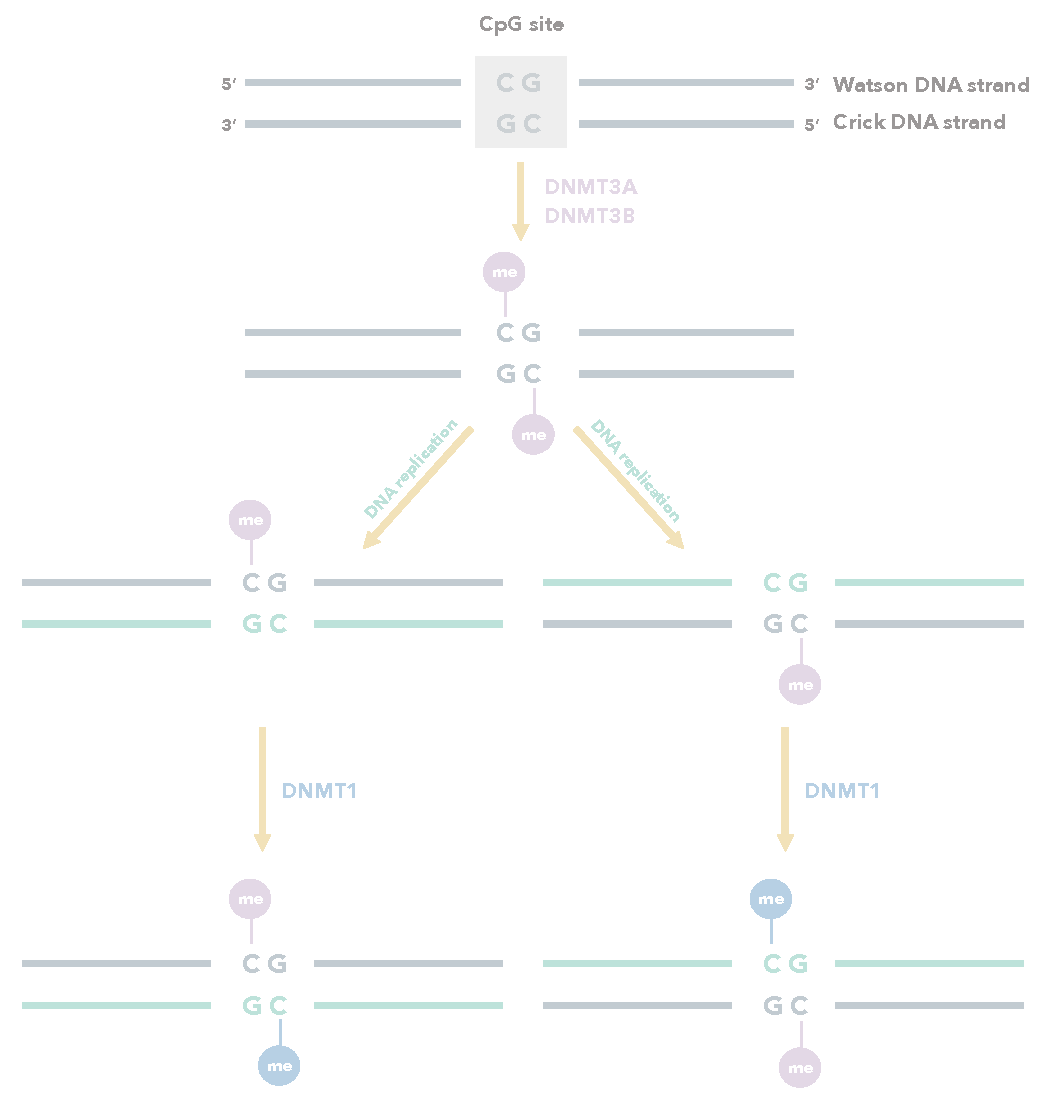
\includegraphics[width=1\textwidth]{C1_Fig3}
	\vspace*{1 mm}
	\caption[Establishment and maintenance of 5-methylcytosine in mammalian genomes]{Establishment and maintenance of 5-methylcytosine (\acrshort{5mC}) in mammalian genomes. Unmethylated cytosines in symmetric CpG sites are originally methylated \textit{de novo} by DNA methyltransferases DNMT3A and DNMT3B to form \acrshort{5mC}. After cell division, the newly synthesised DNA strands lack the methylation mark. Maintenance DNA methyltransferase DNMT1 recognises this hemimethylated DNA and adds the missing methyl groups, therefore ensuring the inheritance of DNA methylation patterns and cellular memory.}
	\label{fig:c1_fig3}
\end{figure}

\bigskip

It was a long-standing question whether the loss of 5mC (a.k.a demethylation) can only occur by replication-coupled passive loss (i.e. preventing DNMT1 maintenance activity and diluting 5mC content by cell division), due to methyltransferase errors or as a result of DNA repair after DNA damage \cite{Iurlaro2017}. In 2009, two groups conclusively identified the presence of a different type of DNA modification in mouse and human DNA, 5-hydroxymethylcytosine (\acrshort{5hmC}) \cite{Kriaucionis2009,Tahiliani2009} (although, surprisingly, its presence in rat tissue had been detected almost 40 years before) \cite{Penn1972}. Furthermore, one of them demonstrated that the enzyme TET1 is capable of oxidising 5mC to 5hmC \cite{Tahiliani2009}. Since then, other enzymes from the TET family (TET2, TET3) have also been shown to catalyse this reaction \cite{Ito2010}. Further products of oxidation, 5-formylcytosine (\acrshort{5fC}) and 5-carboxylcytosine (\acrshort{5caC}), can also be generated by TET enzymes, although their abundance is incredibly low in the genome. Replication-dependent dilution of oxidised products or thymine DNA glycosylase (\acrshort{TDG})-mediated excision of 5fC and 5caC coupled with \acrshort{BER} have been shown to complete the demethylation process (Fig.~\ref{fig:c1_fig4}). Altogether, this shows that \textbf{active enzymatic DNA demethylation is a feature of mammalian epigenomes} \cite{Wu2017}. Finally, it is worth mentioning that another type of DNA modification, N$^6$-methyladenine, has recently been identified in both mouse and human cells, thus further expanding the DNA alphabet \cite{Wu2016,Xiao2018}.

\begin{figure}[htbp!] 
	\centering    
	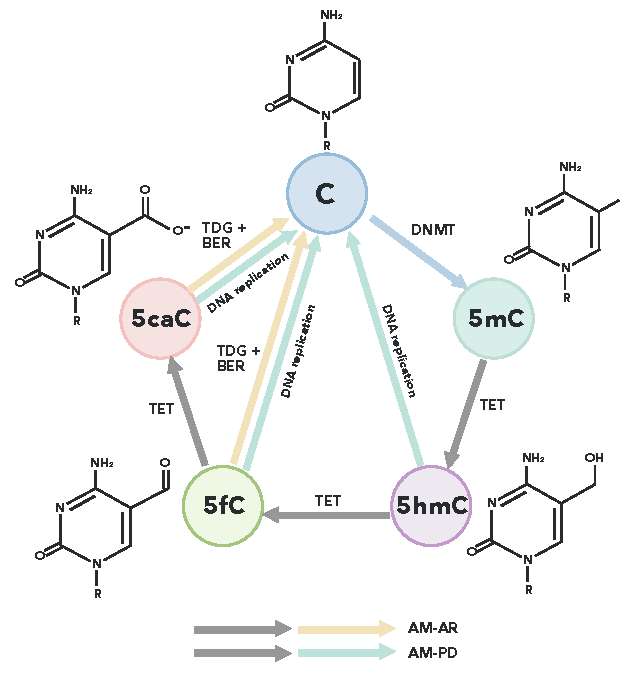
\includegraphics[width=0.8\textwidth]{C1_Fig4}
	\vspace*{1 mm}
	\caption[Oxidation of 5-methylcytosine and the cycle of demethylation]{Oxidation of 5-methylcytosine (5mC) and the cycle of demethylation. 5mC can be oxidised to different DNA modifications (5hmC, 5fC, 5caC) by TET enzymes. The maintenance DNA methyltransferase DNMT1 can only recognise 5mC. As a consequence, after DNA replication, the rest of the modifications would be eventually lost (active modification–passive dilution or AM-PD). Alternatively, thymine DNA glycosylase (\acrshort{TDG})-mediated excision of 5fC and 5caC coupled with base excision repair (\acrshort{BER}) can lead to the same outcome (active modification–active removal or AM–AR). This figure was adapted from \cite{Wu2017}.}
	\label{fig:c1_fig4}
\end{figure}

\bigskip

\textbf{DNA methylation patterns change drastically during mammalian embryonic development}. After fertilisation, mouse and human zygotes undergo epigenetic reprogramming in order to reset naive pluripotency. This is mainly characterised by a global loss of 5mC (i.e DNA hypomethylation) with different demethylation processes affecting the paternal and maternal genome. Nevertheless, some genomic regions, such as imprints, survive epigenetic reprogramming. \textit{De novo} DNA methylation occurs after implantation of the blastocyst, which will restore DNA methylation levels for most somatic cells and eventually generate cell-type specific DNA methylation patterns \cite{Iurlaro2017,Tang2016,Atlasi2017}. 

\bigskip

In the case of the cells that will give rise to the germline (\textbf{primordial germ cells} or \acrshort{PGCs}), further genome-wide DNA demethylation occurs, which makes \acrshort{PGCs} the most hypomethylated cells found during mammalian development thus far (global methylation levels are $\sim$4\%). This ensures imprint erasure and that parental epigenetic memories are removed, therefore posing a barrier for transgenerational epigenetic inheritance. Nevertheless, some regions that escape epigenetic reprogramming in mice and humans have been described (mainly evolutionarily young and potentially hazardous retrotransposons). Methylation patterns of the germline will then be re-established in a sex-specific manner \cite{Tang2016}.  

\bigskip

Over the years, many \textbf{technologies have been developed to measure 5mC and its oxidative products} (see section~\ref{s:4.1} for an overview). Many assays rely on a chemical procedure called bisulfite conversion \cite{Frommer1992}. Genomic DNA is denatured and incubated with sodium bisulfite. This leaves 5mC residues intact, but unmethylated cytosines are deaminated and converted to uracil. Therefore, after PCR amplification, 5mCs are substituted by cytosines while unmethylated cytosines become thymines. This information can then be read at base-pair resolution through DNA sequencing or by hybridisation to a methylation array (such as the Illumina Infinium BeadChips, which are the platform used to generate the data analysed in this thesis) \cite{Plongthongkum2014}. It is important to keep in mind that 5hmC is also resistant to bisulfite conversion, and therefore it is confounded with the 5mC signal \cite{Wu2017}. Furthermore, C>T mutations (a common mutation during ageing, see section~\ref{s:1.1.3}) can be confounded with hypomethylation events. Another caveat of bisulfite treatment is that it degrades DNA to a great degree and generates sequencing libraries of low complexity, which leads to reduced mapping rates and higher costs. A few months ago, Liu \textit{et al.} published a bisulfite-free protocol for 5mC sequencing at base-pair resolution, which could potentially solve some of these issues and start a new generation of bisulfite-free methods \cite{Liu2019}. 

\bigskip

Exposure to certain \textbf{environmental factors is associated with changes in the methylome} that can potentially modulate disease risk. In mice, \textit{in utero} undernourishment leads to weight and metabolic defects in the F$_1$ offspring. Furthermore, this metabolic phenotype is inherited in the F$_2$ offspring through the paternal line. Interestingly, this could be caused because genomic regions that become hypomethylated during paternal germline specification survive epigenetic reprogramming in the F$_2$ zygote and lead to further chromatin alterations in adult tissues \cite{Radford2014}. In a different example, smoking exposure in humans changes DNA methylation patterns of blood \cite{Roby2016} or buccal cells \cite{Teschendorff2015} in a consistent and reproducible manner. However, the mechanisms behind these changes and whether they are functional or mere passenger epimutations remain obscure. Finally, many complex diseases, such as rheumatoid arthritis or many cancer types, are characterised by altered DNA methylation patterns, which suggests that epigenetic mechanisms integrate genetic and environmental aetiologies of disease \cite{Liu2013,Widschwendter2018}.

\smallskip

\subsection{Links between the epigenetic machinery and ageing} \label{s:1.2.3}

\smallskip

As previously mentioned in section~\ref{s:1.1.3}, \textbf{epigenetic alterations are one of the hallmarks of mammalian ageing} \cite{Lopez-Otin2013}. Given the role of genetic pathways and environmental factors in the regulation of organismal lifespan, the epigenetic layer of biological information has attracted a lot of interest in the ageing field (to the point that some authors have suggested that it is the hub that connects all the hallmarks of ageing) \cite{Booth2016}. Indeed, many life-extending interventions (such as dietary restriction, exercise or a robust circadian rhythm) modulate the epigenetic machinery and induce chromatin changes \cite{Benayoun2015a}. Furthermore, since many epigenetic marks are stable over time, they could behave as cellular memories that store past environmental exposures. Taking into account the vast literature available on this topic, in this section I will try to extract the pieces of information that are more relevant for this work.

\bigskip

Several authors have reviewed the wide variety of chromatin changes that occur during ageing in different organisms \cite{Booth2016,Benayoun2015a,Pal2016,Sen2016}. These include changes in histone numbers, histone variants, histone modifications, DNA modifications, non-coding RNAs or nucleosome positioning; which eventually lead to transcriptional deregulation. Certain \textbf{mutations in proteins of the epigenetic machinery affect the lifespan of organisms from yeast to mouse}, thus proving a causal role for some of these changes in the ageing process. Furthermore, I highlight a few interesting insights from these studies:

\begin{itemize}
	
	\item Global heterochromatin loss and redistribution has been suggested as one of the mechanisms behind the ageing process \cite{Villeponteau1997, Tsurumi2012}. Indeed, mutations in proteins that cause premature ageing in humans (such as nuclear lamins or the WRN helicase) have a major impact in heterochromatin structure and the genomic distribution of its characteristic repressive chromatin marks (such as H3K9me3 or H3K27me3) \cite{Zhang2015b}. Cellular senescence is also associated with the remodelling of heterochromatin \cite{Zhang2007}. Furthermore, heterochromatin deregulation can lead to the activation and mobilisation of transposable elements during mammalian ageing \cite{DeCecco2013}. 
	
	\item Mutations that alter the levels of H3K27me3 and H3K4me3 can have contradictory effects in the lifespan of model organisms, probably depending on the loci and cell types that they affect. However, it appears that mutations that increase the levels of H3K36me3 consistently increase lifespan (at least in yeast, worm and fly) \cite{Booth2016,Benayoun2015a,Pal2016,Sen2016}. This will be of interest for Chapter~\ref{c:3}.
	
	\item Increased levels of SIRT6, an H3K9ac and H3K56ac histone deacetylase from the sirtuin family, can extend lifespan of male mice \cite{Kanfi2012}. On the contrary SIRT6-deficient mice die at about 4 weeks, have a progeroid phenotype  and have increased genomic instability (due to problems in the base excision repair pathway) \cite{Mostoslavsky2006}. The role of SIRT6 in human ageing is still not clear. 
	
	\item Histone chaperone ASF1, which promotes histone deposition and stability, is required for normal replicative lifespan in yeast \cite{Feser2010}. Intriguingly, the mouse ortholog ASF1A is important to resolve bivalent chromatin upon differentiation of embryonic stem cells \cite{Gao2018} (see discussion regarding the importance of bivalent domains during mammalian ageing in the `Hypermethylated regions' section below).
	
	\item The naked mole rat, an incredibly long-lived rodent with very low cancer incidence, presents a stable epigenome that is resistant to \textit{in vitro} reprogramming. Furthermore, higher levels of repressive chromatin marks (such as H3K27me3) are observed relative to the mouse \cite{Tan2017}. 
	
\end{itemize}

Importantly, the DNA methylation landscape also seems to be affected during ageing in mammals. Certain CpG sites or genomic regions gain methylation with age (i.e. they become hypermethylated) while others sites lose methylation (i.e. they become hypomethylated). Furthermore, some of these age-associated methylation changes are shared across tissues, while others are tissue-specific. Notably, even though they have an stochastic component, the genomic context where these changes occur seems to be conserved in mice \cite{Maegawa2010,Avrahami2015,Wang2017,Cole2017,Sziraki2018} and humans \cite{Rakyan2010,Teschendorff2010,Horvath2012,Heyn2012,Day2013,Raddatz2013,Weidner2014,Fernandez2015,Dozmorov2015,Yuan2015,Slieker2016,Slieker2018,Zhu2018}:

\begin{itemize}
	
	\item \textbf{Hypermethylated regions}. They are generally enriched for bivalent chromatin, regions repressed by \acrshort{PRC2} (Polycomb Repressing Complex 2) and CpG islands (\acrshort{CGI}s, many of which overlap with bivalent promoters). Bivalent domains are populated with numerous transcription factor binding sites and are marked simultaneously by histone marks H3K27me3 (established by EZH2, which is part of the PRC2 complex; associated with transcriptional repression) and H3K4me3 (established by Trithorax-group proteins; associated with transcriptional activation). The two histone marks seem to co-occur on the same loci of the same cell in a majority of the bivalent domains (as opposed to an heterogeneous population of cells with different histone marks), and sometimes even on the different histone copies of the same nucleosome \cite{Voigt2013}. This opposing duality is thought to silence developmental genes in embryonic stem cells (and pluripotent stem cells in the embryo) while keeping them poised for activation (by developmental and/or environmental cues) \cite{Voigt2013}. Developmental genes (many of them lowly expressed transcription factors) are indeed highly enriched in these regions and this seems to be a feature of most gene ontology analysis performed in hypermethylated CpGs during ageing. Many of the bivalent domains disappear after differentiation, leaving only one of the two marks \cite{Bernstein2006}, but specific nonpluripotent bivalent domains can also be generated after differentiation \cite{Voigt2013}. Besides differentiation, the physiological ageing process also seems to change the landscape of bivalent domains, as observed in aged haematopoietic stem cells or \acrshort{HSCs} (where around 335 bivalent domains disappear in old mouse HSCs, whereas 1,245 emerge) \cite{Sun2014x}. This process is apparently linked to the proliferative history of \acrshort{HSCs} \cite{Beerman2013} and could contribute to the myeloid skewing observed during ageing \cite{Sun2014x,Beerman2013}. Interestingly, bivalent domain loses occur in cancer cells as well, which seems to correlate with the hypermethylation of the regions \cite{Bernhart2016}. It is possible that the ageing- or cancer-related hypermethylation destroys the ability to create a bivalent equilibrium in these regions. If this happens in the stem cells, it could impair adequate differentiation and propagate the methylation change in the tissue. Overall, this provides an interesting mechanistic link between embryonic development, lineage-specific cellular identity and the ageing process that should be further explored.   
	
	\item \textbf{Hypomethylated regions}. They are generally enriched for tissue-specific enhancers (generally marked with H3K4me1) and depleted for \acrshort{CGI}s (which makes sense, given the low methylation levels of CGIs). For example, in wild-type mouse liver, 8230 liver-specific enhancers are hypomethylated during ageing. On the contrary, only 4702 of those enhancers suffer the same fate in Ames dwarf mice (which have decreased insulin/IGF-1 signalling and a longer lifespan), which highlights that the epigenome from Ames dwarf mice appears more stable \cite{Cole2017}.     
	
\end{itemize} 

Importantly, some of these ageing-associated DNA methylation changes also seem to happen in dogs and wolves \cite{Thompson2017}. Furthermore, the rate of change of many of these age-associated regions is negatively correlated with lifespan in six different mammals \cite{Lowe2018}. Altogether, this suggests that conserved epigenetic mechanisms may operate during ageing to shape the mammalian methylome.

\bigskip

Hence, it is clear that the epigenome is eroded over time. In humans, this inter-individual divergence of DNA methylation patterns created upon ageing has been termed `epigenetic drift' \cite{West2013}. Interestingly, this phenomenon is found even in monozygotic twins \cite{Fraga2005,Talens2012}, again highlighting the role of environmental and stochastic factors. This is also observed at the single cell level, where cells from old organisms become more heterogenous at the epigenomic and transcriptomic level \cite{Hernando-Herraez2018,Martinez-Jimenez2017}.

\bigskip

\section{The epigenetic ageing clock}

\subsection{Measuring the ageing process}

\smallskip

In order to study any phenomena one needs to be able to measure it. Using \textbf{survival curves} (a.k.a lifespan curves, i.e. plotting the survival fraction over time, see equation~\ref{eq:1.1}) we have been able to quantify the ageing process at a population level (where the assumption is that life extension in a significant proportion of the population is a surrogate marker of slowed ageing) \cite{Johnson2013}. The adoption of this methodology in model organisms (that we can manipulate genetically and/or pharmacologically) triggered the discovery of the first genes impacting upon the ageing process (i.e. the mutants showed `shifts' of the survival curve when compared with a control). Since then, this has been the main paradigm in ageing research, with efforts being made to automate the process and increase its throughput \cite{Stroustrup2013}.

\bigskip

Nevertheless, measuring the ageing process at the organismal level has proven more difficult. Due to environmental and stochastic factors, there are significant differences in the lifespan of even isogenic organisms. Therefore, there is a real need to develop accurate \textbf{biomarkers of ageing} i.e. measurements of `age-related change(s) in body function(s) or composition that can predict the future onset of age-related disease(s) and/or the residual lifetime left (i.e. predict the rate of ageing) more accurately than chronological age' \cite{Burkle2015a}. Furthermore, according to the American Federation of Aging Research, any valid biomarker of ageing must also monitor a basic (sub)process underlying ageing, it must be able to be tested repeatedly without harming the organism (i.e. it has the potential to become a longitudinal biomarker) and be reproducible in both humans and laboratory animals (such as mice) \cite{Burkle2015a}.

\bigskip

The derivation of a biomarker of ageing leads to the definition of two types of age:

\begin{itemize}
	
	\item \textbf{Chronological age}. It is the time elapsed since the birth of an individual.
	
	\item \textbf{Biological age}. It is the result derived from a specific biomarker. Each biomarker is trained using a set of biological parameters (independent variables) to predict a dependent variable (e.g. chronological age) that captures the probability of dying at a given time. The training takes place using several individuals, ideally from multiple populations. Afterwards, given a new individual and the biological parameters, the biological age can be predicted (and it should capture the risk of death more accurately than chronological age). Younger biological ages should be linked to high fitness and health whereas older biological ages should correlate with age-related disease onset and morbidity \cite{Benayoun2015a}. For example, if chronological age is used as the dependent variable (which is the case for most biomarkers), the biological age of an individual represents the chronological age of the average population that is most similar to the individual (according to the set of biological parameters). In this case, if the biological age of an individual is smaller than his chronological age, this could be interpreted as his probability of death being smaller than the probability of death for the average population (i.e. potentially the rate of ageing of the individual is slower than the average). 
	
\end{itemize}

In the case of humans, the initial ageing biomarkers included traditional biological parameters such as body mass index, waist and hip circumference, blood pressure or heart rate. Over the years, biomarkers that use molecular parameters have also been developed; these include clinical chemistry parameters (such as cholesterol, immunoglobulins or fasting glucose), telomere length or `omics'-based measurements \cite{Burkle2015a,Jylhava2017}. In the latter category, almost every layer of biological information can be used to derive a biomarker, including epigenomics (see next section), transcriptomics \cite{Peters2015a}, proteomics \cite{Tanaka2018}, metabolomics \cite{Hertel2016}, microbiome \cite{Galkin2018} or even brain neuroimaging data \cite{Cole2017a}. Furthermore, composite biomarkers (that combine the biological parameters from molecular layers with measurements of physiological function) \cite{Khan2017} and algorithmic innovations (such as deep neural networks) \cite{Putin2016} will likely improve the predictions. The \textbf{biomarkers of the human ageing process} will serve as personalised risk indicators and will allow monitoring the response to interventions, therefore creating endpoints in clinical trials that target the ageing process.

\smallskip

\subsection{The landscape of epigenetic clocks}

\smallskip

\textbf{Epigenetic clocks} are mathematical models that predict the biological age of an organism using DNA methylation data. These models exploit the fact that DNA methylation patterns change robustly with age in different tissues and species, as summarised in section~\ref{s:1.2.3}. Epigenetic clocks have emerged in the last few years as the most accurate biomarkers of the ageing process in humans, which they can track across the entire lifespan. As a quick comparison, telomere length (one of the other popular ageing biomarkers) achieves a Pearson's correlation coefficient with chronological age of $\sim$ -0.5 in blood leukocytes in the best case scenarios (with many studies reporting much lower values and contradictory results) \cite{Newman2013}. On the other hand, the coefficients for Hannum's or Horvath's epigenetic clocks (discussed later) are generally above $\sim$ 0.8 (in virtually all studies assessed) \cite{Chen2016}.

\bigskip

The idea that DNA methylation patterns behave in a clock-like manner during cellular ageing was already proposed by Holliday and Pugh in 1975 \cite{Holliday1975}. With the advent of high-throughput DNA methylation technologies, some authors started to test the \textbf{ability of DNA methylation patterns to predict chronological age in humans}. In 2010, Bork \textit{et al.} showed that DNA methylation values change at specific CpG sites upon long-term culture and between young and old individuals in mesenchymal stromal cells \cite{Bork2010}. Later that same year, studies by Teschendorff \cite{Teschendorff2010}, Rakyan \cite{Rakyan2010}, Gronninger \cite{Gronniger2010} and others identified sets of CpG sites (signatures) that consistently altered their methylation states with age in different tissues and cell types (and interestingly some of them seemed to occur in the same genomic context). In 2011, Bocklandt \textit{et al.} demonstrated that it was possible to predict chronological age in saliva with an average error of 5.2 years using the DNA methylation values of only two CpG sites \cite{Bocklandt2011}. Shortly afterwards, Koch \textit{et al.} built what was probably the first multi-tissue predictor of chronological age in humans (which worked using the same 5 CpG sites across different cell types) \cite{Koch2011}. 

\bigskip

The potential role of epigenetic clocks as biomarkers of human ageing was probably realised after the publications, in 2013, of the models by Hannum \textit{et al.} \cite{Hannum2013} and Horvath (Table~\ref{tab:clocks}) \cite{Horvath2013}. Since then, these epigenetic clocks have being validated in a large number of independent cohorts and have become, \textit{de facto}, the default human epigenetic clocks for blood and multi-tissue predictions respectively. Importantly, this inspired other groups to build epigenetic clocks in the mouse \cite{Wang2017,Stubbs2017,Petkovich2017,Thompson2018,Meer2018}, dogs and wolves \cite{Thompson2017} or even humpback whales \cite{Polanowski2014}; which will be instrumental to broaden our understanding of the biology of ageing in mammals \cite{Stubbs2017}. A comparison of some of these epigenetic clocks can be found in Table~\ref{tab:clocks}. The accuracy that they can achieve with a relatively small number of CpG sites as covariates is remarkable.

\bigskip

The predictions from epigenetic clocks are normally referred as epigenetic age (which is equivalent to the concept of biological age previously explained). Interestingly, deviations of epigenetic age from chronological age (a.k.a \textbf{epigenetic age acceleration} or \acrshort{EAA}) have been associated with many conditions in humans, including time-to-death \cite{Chen2016,Marioni2015}, HIV infection \cite{Horvath2015b}, Down syndrome \cite{Horvath2015a}, obesity \cite{Horvath2014}, menopause \cite{Levine2016} and breast-cancer risk in women \cite{Kresovich2019}, Werner syndrome \cite{Maierhofer2017} or Huntington’s disease \cite{Horvath2016a}, among others (reviewed in \cite{Horvath2018}). Interestingly, females and people of Hispanic ethnicity have lower \acrshort{EAA} (after correcting for blood cell composition effects) when compared with males and those of Caucasian origin respectively, highlighting a role for biological sex and genetic background in the rate of the epigenetic ageing clock \cite{Horvath2016}. In mice, the epigenetic clock is slowed down by dwarfism and calorie restriction \cite{Wang2017,Cole2017,Petkovich2017,Thompson2018,Meer2018} and is accelerated by ovariectomy and high fat diet \cite{Wang2017,Stubbs2017, Petkovich2017,Thompson2018}. 

\bigskip

\begin{table}
	\begin{tabular}{p{3.5cm} | p{2.5cm} p{2.5cm} p{2.5cm} p{2.5cm}}
		\toprule 
		\textbf{Species} & Human & Human & Mouse & Dog and wolf \\
		\midrule
		\textbf{Main reference} & Hannum \textit{et al.} \cite{Hannum2013} & Horvath \cite{Horvath2013} & Stubbs \textit{et al.} \cite{Stubbs2017} & Thompson \textit{et al.} \cite{Thompson2017} \\
		\midrule
		\textbf{DNA methylation technology} & Illumina methylation array (450K) & Illumina methylation array (27K and 450K) & RRBS & RRBS \\
		\midrule
		\textbf{N samples (in training set)} & $N=482$ & $N=3931$ & $N=129$ & $N=108$ \\
		\midrule
		\textbf{Tissues (in training set)} & Blood & Multi-tissue (18) & Multi-tissue (7) & Blood \\
		\midrule
		\textbf{Age range (in training set)} & 19-101 years & 0-100 years & 1-41 weeks & 0.5-8 years \\
		\midrule
		\textbf{Number of CpGs in the final model} & 71 & 353 & 329 & 115 \\
		\midrule
		\textbf{Median absolute error (\acrshort{MAE})} & 4.9 years & 3.6 years & 3.33 weeks & 0.8 years \\
		\midrule
		$\frac{MAE}{max.\ age\ in\ model} \cdot 100$ & 4.85\% & 3.6\% & 8.12\% & 10.0\% \\    
		\bottomrule 
	\end{tabular}
	\vspace*{3mm}
	\caption[Comparison of epigenetic clocks in different species]{Comparison of some of the epigenetic clocks available for different species. \acrshort{RRBS}: reduced representation bisulfite sequencing (see Chapter~\ref{c:4}).}
	\label{tab:clocks}
\end{table}  


Recently, \textbf{other epigenetic clocks} have been created for slightly different purposes. For example, Yang and colleagues developed an epigenetic clock that can track the rate of (stem) cell divisions in normal and cancerous tissue (see section~\ref{s:2.3.2}) \cite{Yang2016}. Furthermore, an epigenetic clock that performs well in skin cells (such as fibroblasts, buccal cells and endothelial cells; known as the skin-blood clock) was developed in order to improve \textit{ex vivo} studies or forensic applications \cite{Horvath2018a}. Moreover, this epigenetic clock enables the detection of \acrshort{EAA} in Hutchinson-Gilford progeria, which is not possible with Horvath's clock \cite{Horvath2018a}. Additionally, other epigenetic clocks have been trained to predict more complex dependent variables than chronological age. Levine \textit{et al.} built a model that predicts a combination of chronological age with clinically-relevant variables (such as erythrocytes distribution width or serum glucose), known as \textit{PhenoAge} \cite{Levine2018}; while Lu \textit{et al.} built a model that predicts a composite variable mixing information from smoking pack-years and plasma proteins (adrenomedullin, C-reactive protein, plasminogen activation inhibitor 1 and growth differentiation factor 15), known as \textit{GrimAge} \cite{Lu2019}. These models perform better than previous epigenetic clocks in predicting the onset of several age-related diseases and therefore they will likely be useful in a clinical context.    

\bigskip

From an statistical point of view, most of the epigenetic clocks have been built using linear regression (see section~\ref{s:2.4}). A model needs to be trained to predict the dependent variable (normally chronological age) using the methylation values of different cytosines (generally in CpG context) as covariates. Given that the number of covariates is normally several orders of magnitude bigger than the number of samples available for training, regularisation (i.e. `shrinking' of the linear regression coefficients, many of which become zero) needs to be performed. More specifically, elastic net (a combination of lasso and ridge regularisation) has been successfully applied \cite{Friedman2010}. \textbf{Many epigenetic clocks with similar performance can be built from different sets of CpG sites} (i.e. the construction of epigenetic clocks is highly statistically degenerate) \cite{Thompson2018}. Therefore, it is important to understand that the CpG sites that constitute an epigenetic clock are not necessarily the most important biologically, but rather they are probably a lower-dimensional representation of the main processes that shape the epigenome with age.


\smallskip

\subsection{Molecular mechanisms of the epigenetic ageing clock} \label{s:1.3.3}

\smallskip

At this point it is probably useful to clarify a few concepts that I will refer to throughout this work. I define the \textbf{epigenetic ageing clock} as the biological mechanisms that give rise to the genome-wide epigenetic changes that occur during ageing (in a given species); a definition in line with the one reported in \cite{Horvath2018}. These changes have been widely studied in the context of DNA methylation and can be utilised to train predictors of chronological age (or other more complex variables). These predictors constitute different types of \textit{epigenetic clocks}, and I will try to refer to them by the specific model being mentioned (e.g. Horvath's epigenetic clock, Hannum's epigenetic clock, etc.). As such, specific epigenetic clocks capture the changes associated with the underlying epigenetic ageing clock.

\bigskip

The molecular mechanisms that control the rate of the epigenetic ageing clock are still mysterious \cite{Horvath2018,Field2018}. Steve Horvath proposed that his multi-tissue epigenetic clock captures the workings of an \textbf{epigenetic maintenance system}, although the molecular nature of this hypothetical system is unknown to this date \cite{Horvath2013}. Furthermore, we still do not know whether these changes are functional at all or whether they are just downstream consequences of other molecular processes that drive ageing. 

\bigskip

As mentioned in section~\ref{s:1.2.3}, many studies have characterised changes in DNA methylation patterns during mammalian ageing, some of which seemed to be evolutionarily conserved \cite{Lowe2018,Horvath2013}. Interestingly, changes that involve a gain in methylation during ageing seem to be more conserved across tissues, whilst changes involving hypomethylation are generally more tissue-specific \cite{Horvath2013,Yang2016}. Furthermore, many of these changes occur in \textbf{regions normally occupied by Polycomb Repressing Complex 2}, which are marked by the repressive histone mark H3K27me3. Therefore, it is likely that disruptions of H3K27me3 domains (which are generally inherited after cell division) play a role in epigenetic ageing. A specific instance would be bivalent promoters (which are marked by both H3K27me3 and H3K4me3); these tend to gain methylation with age (see section~\ref{s:1.2.3}). These signals are captured by most epigenetic clocks trained to predict chronological age \cite{Horvath2018}.

\bigskip

The mere existence of multi-tissue epigenetic clocks supports the idea that some of the mechanisms behind the epigenetic ageing clock are shared across tissues. Furthermore, Hannum's epigenetic clock (trained exclusively in blood) explains 72\% of variation in chronological age across other tissues (such as breast, kidney, lung and skin), although there is generally a tissue-specific offset \cite{Hannum2013}. Interestingly, Horvath's epigenetic clock (which is multi-tissue) presents positive epigenetic age acceleration in breast tissue \cite{Sehl2017}, whilst the cerebellum looks younger than expected \cite{Horvath2015} and some tissues are poorly calibrated (uterine endometrium, dermal fibroblasts, skeletal muscle and heart) \cite{Horvath2013}. Moreover, Horvath's epigenetic clock dramatically underestimates epigenetic age in sperm \cite{Horvath2013}, which highlights differences between somatic cells and the germline. Altogether, this raises the possibility that \textbf{some of the mechanisms behind the epigenetic ageing clock may be shared across tissues} but that they may operate at different rates (e.g. because of different exposure to hormones, differences in proliferation rate, etc.). 

\bigskip

Horvath's epigenetic clock works in primary tissues and cell types, and also \textit{in vitro} (both in cell culture and organoids) \cite{Horvath2013,Hoshino2019}. Furthermore, recipients of allogeneic hematopoietic stem cell transplantations show an epigenetic age in their blood that corresponds to the age of the donor, even 17 years after the transplantation took place \cite{Soraas2019}. This suggests that \textbf{the epigenetic ageing clock is a stable cell-intrinsic property}, as opposed to the idea that it is highly influenced by the systemic environment (such as the effects observed in heterochronic parabiotic experiments) \cite{Conboy2005}. The stability is further demonstrated by experiments showing that human fibroblasts that have been reprogrammed into neurons maintain their original epigenetic age \cite{Huh2016}.     

\bigskip

Epigenetic age acceleration (\acrshort{EAA}) has been proposed as a way to capture the ageing phenotype in GWAS analysis. Genetic variants associated with \acrshort{EAA} have been found in \textit{TERT}, the catalytic subunit of telomerase \cite{Lu2018}. Epigenetic age increases \textit{in vitro} with cell passage, but it requires the expression of \textit{TERT} to keep linearly increasing after a certain number of passages \cite{Lu2018}. This suggests that bypassing replicative senescence is required for the epigenetic ageing clock to keep ticking, at least \textit{in vitro}. Interestingly, inducing senescence in TERT-immortalised cells via an oncogene makes the cells age faster in culture, but induction of senescence via DNA damage does not increase epigenetic age \cite{Lowe2016}. Overall, this could imply that \textbf{the epigenome of senescent cells does not contribute substantially to the changes captured by the epigenetic ageing clock}. Furthermore, it has been proposed that epigenetic ageing could serve a complementary role to that of senescence, by suppressing potential cancer development (e.g. by protecting against dedifferentiation signals) \cite{Horvath2018}. The molecular connections between cell division (positive \acrshort{EAA} is generally found in cancerous tissue) \cite{Hannum2013,Horvath2013}, alternative non-telomeric functions of \textit{TERT} and the epigenetic ageing clock need to be further studied. Moreover, these experiments do not discard an indirect effect of senescent cells on the epigenetic ageing clock (i.e. via the \acrshort{SASP} by inducing changes in the epigenomes of other cells in the tissue) that could occur \textit{in vivo}. 

\bigskip

The rate of the epigenetic ageing clock is substantially faster during post-natal organismal growth (something that Horvath's model accounts for) \cite{Horvath2013}, which could be related to the high levels of \textit{TERT} expression during this period \cite{Lu2018}. Interestingly, epigenetic ageing according to Horvath's epigenetic clock (but not according to other epigenetic clocks, such as Hannum's clock, the skin-blood clock, $PhenoAge$ or $GrimAge$) seems to start a few weeks post-conception in fetal tissues \cite{Hoshino2019}. This could imply that the molecular processes responsible for mammalian epigenetic ageing are operative even during pre-natal development, potentially with different consequences. 

\bigskip

This \textbf{molecular continuum between development and ageing} is further reinforced by the fact that embryonic stem cells have an epigenetic age around zero \cite{Horvath2013}. Notably, \textit{in vitro} reprogramming of somatic cells into induced pluripotent stem cells (\acrshort{iPSCs}) also reduces epigenetic age to values close to zero (or even negative) both in humans \cite{Horvath2013} and mice \cite{Petkovich2017,Meer2018}. Moreover, the induction of \textit{in vivo} partial reprogramming (short and cyclic exposure to reprogramming factors) in progeric mice ameliorates several ageing phenotypes and extends lifespan \cite{Ocampo2016}. We are currently testing whether a similar protocol applied to physiologically aged mice can reduce epigenetic age. This is of extreme importance since it shows that the epigenetic changes associated with the epigenetic ageing clock are reversible, which opens the door to further mechanistic studies and to the development of rejuvenation therapies \cite{Rando2012,Olova2019,Mahmoudi2019,Sarkar2019}.

\bigskip

The goal of this thesis is to improve our understanding of the epigenetic ageing clock in humans. For this purpose, I will first review statistical methods to quantify epigenetic ageing in human blood (Chapter~\ref{c:2}). Then, I will study how different proteins of the epigenetic machinery affect the rate of the epigenetic ageing clock (Chapter~\ref{c:3}). Next, I will discuss a technological improvement with the potential to make future epigenetic clocks more cost-effective (Chapter~\ref{c:4}). Finally, I will provide interesting future avenues that should be explored in order to unravel the molecular mechanisms of the epigenetic ageing clock (Chapter~\ref{c:5}). 
